\documentclass[a4paper, % papirstørrelse, skal altid med
final,% Når man skal skifte kompileringsmetode mellem draft og final skal man 
      %flytte kommenteringen %  i Draft kommanoerne, nedenfor.
11pt, % standardstørrelse på fonten
openany%, % anvnedes hvis kapitler bare skal starte på den næste side
%oneside,
%article
]{memoir}%
% marginer, memoir to to metoder
% den traditionelle, se memoir manualen
% venstre: 2.5cm, højre: 3.5cm, top: 3cm, bund: 4cm
%her kan margenen sættes manuelt, hvis man har lyst
%\setlrmarginsandblock{3.5cm}{3.5cm}{*}
%\setlrmarginsandblock{1.5cm}{6.5cm}{*}
%her kan margenen sættes manuelt, hvis man har lyst
%\setulmarginsandblock{3cm}{4cm}{*}
% % mere utraditionelt, men hurtigt smartere
% % vi sætter tekstblokken og placerer den
% % værdierne som er angivet svarer ca. til dem anvende i LaTeXbogen
% % 400pt bred og en højde svarende til at forholdet er det gyldne snit
%\settypeblocksize{*}{300pt}{1.618}
% % placer tekstblokken på papriet, kun en værdi skal angives, her sider
% % vi bare hvad forholder mellem marginerne skal være
% \setlrmargins{*}{*}{1.6}
% \setulmargins{*}{*}{1.3}
\checkandfixthelayout % laver forskellige beregninger og sætter de
% almindelige længder op
\usepackage[utf8]{inputenc} % eller utf8 eller ansinew eller ...
\usepackage[danish]{babel} %direktiv til at bruge det danske sprog

\usepackage[draft]{fixme} % til at skrive \fixme kommentarer til sig

%\newenvironment{Draft}{\fixme{HUSK at ændre kommenteringen i preamble når man skifter mellem draft og final} }{  }
\let\Draft=\comment \let\endDraft=\endcomment


%har vi ord der bliver delt forkert kan de indsættes i hyphernation med bindestreg alle steder hvor ordet kan deles
\hyphenation{tit-len mo-del-len pro-du-ce-rer an-svars-hav-ende om-for-deles for-bind-elses-mulig-heder ska-ber æn-dring-er net-værks-en-hed-er peer backup backup-system fast-track backup-systemer nabo-peers frame-work efter-som Grund-lag-et plads-effek-tivi-teten audits}


\usepackage{nameref}
\usepackage[danish]{varioref} % smarte krydsreferencer via \vref
\usepackage[colorlinks, linkcolor=blue, citecolor=blue, urlcolor=blue, 
final=true]{hyperref}

%giver mulighed for at hoppe i pdf'filen via referencerne.
%hyperref er ustabil med varieof,
%og skal udkommenteres hvis der opstår problemer.
%specielt skal udkommenteres når man kompilere i final til print

\renewcommand\danishhyphenmins{22} % bedre orddeling
\addto\captionsdanish{%brug bedrer danske ord for de faste tekster
\renewcommand\contentsname{Indholdsfortegnelse}
\renewcommand\appendixname{Appendiks}
}

\usepackage{csquotes}
\usepackage[style=numeric-comp,sorting=nyt]{biblatex}
\DefineBibliographyStrings{danish}{%
references      = {Litteraturliste},
bibliography    = {Litteraturliste},
urlseen         = {Lokaliseret d\adddot},
andothers 		= {m\adddot fl\adddot},
typeeditor      = {{udgiver}{udg\adddot}},
typeeditors 	= {{udgivere}{udg\adddot}},
}

\usepackage[T1]{fontenc} % bedre orddeling og ofte påkrævet at
% forskellige fonte
%\usepackage{fourier} % eller mathpazo eller lignende, eller fjern den
% for at få standard fonten
% sætter nogle default værdier vedr. floats

\let\newfloat\relax % memoir har allerede defineret denne men det gør
% float pakken også
\usepackage{float}
\restylefloat{table}
\floatevery{table}{\centering\small} % alle tabel floats centreres og
% skrives i \small
\restylefloat{figure}
\floatevery{figure}{\centering} % automatisk centrering af alle
% figurer
% float environments får ’htbp’ som standard placerings værdier når
% man ikke har angivet noget

\makeatletter
\renewcommand\fps@figure{htbp}
\renewcommand\fps@table{htbp}
\makeatother
\usepackage{amsmath,amssymb} % bedre matematik og ekstra fonte
\usepackage{textcomp} % adgagn til tekstsymboler
\usepackage[notcite,notref]{showkeys} % viser labels i margin,
% udkommenteres for at fjerne, eller
% anvend option final


\setsecnumdepth{subsubsection} % eller hvor dybt man nu ønsker at har
% overskrifterne nummereret
\maxsecnumdepth{subsubsection}
\settocdepth{subsubsection} % hvor dybt ned vi ønsker ting med i

% OPSÆTNING AF SÆTNINGER etc.
\usepackage[amsmath,thmmarks]{ntheorem} % bedre fleksimibitet
\usepackage[final]{graphicx} % pakke til inklusion af grafik
\usepackage{epsfig}

\makeindex % hvis man ønsker at lave et index
%\usepackage{pstricks}
\usepackage{tikz}

%\newcommand{\tightlist}{%
% \setlength{\itemsep}{0pt}
%  \setlength{\parskip}{0pt}}

%Linjeafstand: (1,5 = siderne bliver ca. til ns)
\linespread{1,5} 
\selectfont

\newcommand{\des}[0]{Discrete event simulation }
\newcommand{\ds}[0]{Deadline scheduling }
\newcommand{\is}[0]{Interaktiv scheduling }

 
% OPSÆTNING TIL INKLUDERING AF SOURCE CODE
\usepackage[final]{listings}
\renewcommand{\lstlistingname}{Kodestump}
\renewcommand{\lstlistlistingname}{Kodestumper}
	\usepackage{courier}
 \lstset{ 
         basicstyle=\footnotesize\ttfamily, % Standardschrift
         %numbers=left,               % Ort der Zeilennummern
         numberstyle=\tiny,          % Stil der Zeilennummern
         %stepnumber=2,               % Abstand zwischen den Zeilennummern
         numbersep=5pt,              % Abstand der Nummern zum Text
         tabsize=2,                  % Groesse von Tabs
         extendedchars=true,         %
         breaklines=false,            % Zeilen werden Umgebrochen
         keywordstyle=\color{red},
                frame=b,         
         keywordstyle=[1]\textbf,    % Stil der Keywords
         keywordstyle=[2]\textbf,    %
         keywordstyle=[3]\textbf,    %
         keywordstyle=[4]\textbf,   %\sqrt{\sqrt{}} %
         stringstyle=\color{white}\ttfamily, % Farbe der String
         showspaces=false,           % Leerzeichen anzeigen ?
         showtabs=false,             % Tabs anzeigen ?
         xleftmargin=17pt,
         framexleftmargin=17pt,
         framexrightmargin=5pt,
         framexbottommargin=4pt,
         %backgroundcolor=\color{lightgray},
         showstringspaces=false      % Leerzeichen in Strings anzeigen ?        
 }
 \lstloadlanguages{% Check Dokumentation for further languages ...
         [Visual]Basic,
         Pascal,
         C,
         C++,
         XML,
         HTML,
         PYTHON,
 }
\lstset{language=Python}
\lstset{emph={@process, @choise, Alternation, Skip,Timeout,Parallel,Sequence, Spawn,@io,ChannelPoisonException, ChannelRetireException},emphstyle=\underbar}


    %\DeclareCaptionFont{blue}{\color{blue}} 

  %\captionsetup[lstlisting]{singlelinecheck=false, labelfont={blue}, textfont={blue}}
  \usepackage{caption}
\DeclareCaptionFont{white}{\color{white}}
\DeclareCaptionFormat{listing}{\colorbox[cmyk]{0.43, 0.35, 0.35,0.01}{\parbox{\textwidth}{\hspace{15pt}#1#2#3}}}
\captionsetup[lstlisting]{format=listing,labelfont=white,textfont=white, singlelinecheck=false, margin=0pt, font={bf,footnotesize}}




\usepackage{pdfpages}

%\includeonly{../litteratur}






\title{Peer-to-peer Backup}
\author{Simon Christiano Bognolo og Rasmus Ebdrup Sørensen}
\begin{document}
%\begin{titlingpage}
%\maketitle
%\end{titlingpage}


\frontmatter
\small
\tableofcontents
\normalsize
\newpage


\listoffixmes
 \newpage

%\input{../husk}
\savepagenumber
\mainmatter
\linespread{1,5}
\selectfont
%%%%%%%%%%%%%%%%%%%%%%%%%%%%%%%%%%%%%%%%%%%%%%%%%%%%%%%%%%%%%%%%%%%%%%
%%\chapter{Intro} 
\section*{Problemformulering}
%hvad vi vil lave , hvordan vi vil lave det, hvad det skal resultere i, hvorfor gør vi det. 

Vi ønsker i dette speciale at analysere mulighederne for i praksis at inkludere tre tidsmodeller DES, deadline scheduling og interactive time i pycsp.
%Vi ønsker med eksempler at vise vores udviddelse med praktiske eksempler ledsaget af tegninger og tekst.

Vi ønsker på baggrund af analysen at foretage en hel eller delvis implementation af tidsmodellerne. Med udgangspunkt i eksempler vil vi påvise fordele og ulemper i implementationen, samt foretage en sammenligning med den hidtidige måde at simulere tid på.

Vi ønsker at vores udvidelse skal kunne bruges i et bredere udviklermiljø, og derfor ønsker vi at vores løsning skal være teknisk velfunderet samt have en notation der nemt kan bruges.

%Vi ønsker at udvidde sproget pycsp så det i praksis bliver muligt for processer at kende til tid.
\subsection*{Motivation}
For at modellere de nævnte tidsmodeller i PyCSP idag, er en meget benyttet metode at introducerer barrierer for at definere tidsskridt. Denne løsning kræver en stor omskrivning af et udviklet program, sammenlignet med en version uden en tidsmodel. Dette er ikke ønskværdigt og vi vil gerne udvikle en funktionalitet i PyCSP, så man kan benytte tid intuitivt i et udviklet program.

Der er tidligere blevet arbejdet med at introducere tid i CSP, specifikt i form af Timed CSP. Dette er dog primært et teoretisk arbejde, og har aldrig vundet indpas som en gnængs standtard i praktiske implementationer af CSP. 
Vi tror at en praktisk anvendelig implementation af tidsbegrebet vil have stor betydning for PyCSP's anvendelighed og udbredelse som et værktøj til at løse problemer der naturligt har en dimension af tid. 

\fxnote[inline]{Skal vi komme ind på at man med tid vil kunne resonere om processerne ud fra en stokastisk tidselement.}

\fxnote{Brian kan du komme med mere motivation.}

\subsection*{Resultat}
Projektet skal resultere i en udviddelse af PyCSP der understøtter de nævnte modeller, samt en evaluering af udviddelsen. En vigtig del af resultatet vil være en række forklarende eksempler, der viser ''best practice'' for anvendelsen.
\\
\\
\textbf{Læringsmålene for dette projekt er som følger:}

\begin{itemize}
 \item Identificere problemstillingerne ved at introducere tidsmodeller i PyCSP.
 \item Argumentere for hvilke ændringer  der skal foretages i PyCSP for at introducere tidsmodeller.
 \item Foretage en hel eller delvis implemention i PyCSP af de nævnte ændringer.
 \item Foretage en evaluering de implementerede tidsmodeller sammenholdt med lignende løsninger.
 \item Beskrive de foretagede ændringer så de er trivielle at benytte for folk med kendskab til PyCSP.
 \item Gennem eksempler demonstrere anvendelsen.
\end{itemize}
\end{document}

%\newpage
\chapter{Eksempler}

\section{Hajer og fisk på Wator} Som eksempel på en DES simulation
har vi valgt at tage udgangspunkt i det scenarie som A. K. Dewdney
beskrev i artiklen \fixme[inline]{reference}. Artiklen beskriver den
fiktive planet Wator, der har form som en torus og er fuldstændig
dækket af vand. Verdenen er inddelt i felter som beskrevet på side
20 i \fixme[inline]{ref}. Disse felter kan være tomme, indeholde en
fisk eller en haj. Følgende karakteristika beskriver fisk og hajers
opførsel.


Fisk - bevæger sig og forplanter sig Lever af plankton, en ressource
som er uendelig. Hvis der er et ledigt tilstødende felt bevæger en
fisk sig til dette felt. Hvis der er flere ledige felter vælges et
tilfældigt. Hvis en fisk overlever 3 livscykler forplanter den sig.


Hajer - jager og forplanter sig Såfremt der er fisk i et eller flere
tilstødende felter flytter hajen sig herhen og spiser fisken. Hvis der
er flere tilstødende felter med fisk vælges et tilfældigt. Er der
ikke nogen fisk i nærheden bevæger en haj sig på samme måde som en
fisk. Hvis en haj ikke spiser i mere end 3 livscykler dør den. Hvis en
haj overlever 10 livscykler forplanter den sig.

For hvert tidsskridt vil alle fisk og hajer udføre en handling ud fra
ovenstående opførsel.

Til at initiere systemet skal der defineres en størrelse af verdenen,
samt hvor mange fisk og hajer der er til stede fra start. Disse fisk og
hajer placeres tilfældigt i verdenen.

Såfremt de initielle parametre understøtter en bæredygtig bestand
forventer vi at se bestanden af henholdsvis fisk og hajer oscillere
afhængigt af hinanden.

\section{Kunder i en bank} Et klassisk eksempel inden for \des

%\newpage
%\input{../litteratur}
%\newpage
\subsection{Scheduler}
Med valget af greenletversionen som grundversionen, og med henblik på at hovedparten af vores ændringer vil være i scheduleren, vil vi kort gennemgå denne.

\begin{lstlisting}[firstnumber=132,stepnumber=5,numbers=left, float, label=fig:scheduling, caption=Uddrag af Scheduler.py i greenletsversionen.]
    def getInstance(cls, *args, **kargs):
        '''Static method to have a reference to **THE UNIQUE** instance'''
        if cls.__instance is None:
            # (Some exception may be thrown...)
            # Initialize **the unique** instance
            cls.__instance = object.__new__(cls)

            # Initialize members for scheduler
            cls.__instance.new = []
            cls.__instance.next = []
            cls.__instance.current = None
            cls.__instance.greenlet = greenlet.getcurrent()

            # Timer specific  value = (activation time, process)
            # On update we do a sort based on the activation time
            cls.__instance.timers = []

            # Io specific
            cls.__instance.cond = threading.Condition()
            cls.__instance.blocking = 0
\end{lstlisting}

 I \cref{fig:scheduling} ses et uddrag af initialiseringskoden. Dels findes der tre lister af processer som scheduleren har mulighed for at vælge imellem når der skiftes proces.  
 \begin{list}
 \tightlist 
 \item \code{new}: Initeres på linje 140, og består af processer som lige er blevet scheduleres for første gang.
 \item \code{next}: Initeres på linje 141, og indeholder de processer der er klar til at blive kørt, og som har været kørt før.  
 \item \code{timers}: Initeres på linje 147, og indeholder de processer der har tilknyttet en timeout. De skal først scheduleres på et senere tidspunkt og venter dermed blot. Hvert element i listen består både af processen samt et tidsstempel for hvornår processen skal genaktiveres. Denne liste bliver gensorteret hver gang der indsættes en ny proces.
 \item \code{blocking}: Initieres på linje 150, og er en variabel.Processer der venter på IO operationer, er ikke klar til at blive scheduleret, men heller ikke afsluttet. Scheduleren kan derfor ikke schedulere dem, men holdes styr på antallet af ventende processer vha. denne variabel, for at kunne afgører om Scheduleren skal afslutte eller afvente.
\end{list}

Når \sched en er startet, itererer den igennem alle tre lister, indtil de alle er tomme, og der ikke er nogle processer der er blokeret. Dette betyder at der ikke længere kan komme processer der ønskes at blive lagt på \sched en, og den kan dermed afslutte.

For at markere at vi ikke kun skal foretage en planlægning
af processerne, men foretage en simulering, har vi lavet en
\code{Simulation} klasse der arver fra \code{Scheduler}. Alle ændringer
vi skal foretage for at gå fra en almindelig \sched ~til en simulerings
\sched, vil således indkapsles i denne klasse, mens alt hvad de to
klasser har til fælles vil være isoleret i greenlets versionen af
\code{Scheduler} klassen. Dette har yderligere den fordel at man tydeligt kan se
at alle klasserne i simulation versionen arver en simulerings \sched ~og
ikke \code{Scheduler} fra greenletsversionen.

%\fxnote{dårlig overskrift}{\subsection{Repræsentation af tid}} Vi
%vil i dette afsnit gå i dybden med listen \code{timers} der findes i
%klassen \code{Scheduler}, samt se hvordan den kan inkorporeres i vores
%design.

\subsection{Tid i greenletsversionen} I \pycsp foregår kommunikation
kun når begge kanalender er klar dvs. når der både findes en
kanalende der vil skrive og en kanalende der vil læse. Hvis
kun en af kanalenderne er klar, vil den vente indtil der findes
minimum en kanalende af hver type, der er klar. Dette medfører
risikoen for at processen aldrig kommer videre, men går i deadlock.
I \pycsp har man derfor i \code{alternation} mulighed for at
tilknytte en timeout til en \code{guard}. Dette giver mulighed for
at en proces, kun er villig til at vente på kommunikation i en
given tidsperiode. 
\begin{lstlisting}[float=hbtp, label=Timeout,caption=Timeout i Alternation (fra dokumentationen til PyCSP)]
Alternation([{Timeout(seconds=0.5):None}, 
             {Cin:None}]).select()
\end{lstlisting}

I \cref{Timeout} ses et minimalt eksempel hvor processen kun er villig
til at læse fra kanalenden \code{Cin} i $0.5$ sekunder. Hvis ikke der
er modtaget en besked indenfor 0.5 sekundt, accepteres timeoutguarden
og processen er ikke længere villig til at læse fra \code{Cin}, og
fortsætter sin kørsel.

Tid er dermed blevet introduceret i \pycsp, men kun for at at have
mulighed for at tilknytte timeout til en \code{alternation}. Vi ønsker
at videreudvikle denne struktur til at håndtere tidsdelen for alle
processer, samt for at fungere med diskret tid, modsat den eksisterende
løsning hvor tiden er kontinuerligt.

\subsection{Timers}  
Vi forventer at brugen af
listen \code{timers}, vil øges betragteligt og at den gennemsnitlige
længde af listen vil stige, når der udvikles simuleringsproblemer. Dermed 
øges kravet om en effektiv implementation af \code{timers}\fxnote{skal 
vi evaluere om dette rent faktisk forbedrer ydelsen}. 

For at forbedre ydelsen af \code{timers} listen, 
ændrer vi den fra en almindelig liste, til en min"-hob. En hob har
flere fordele ved skemaplanlægning og er nævnt i introduktionen til Pythons implementation af en hob\fxnote{ref til http://docs.python.org/dev/3.0/library/heapq.html}. 

Da en implementation af en hob
allerede findes i Pythoni modulet \code{Heapq}, som er effektivt implementeret i C, vælger vi at bruge denne. Den eneste handling
der ikke er som standard er implementeret, er fjernelsen af et arbitrært element
fra hoben. Dette sker i den eksisterende løsning når en proces
aktivere et andet valg i \code{alternation} end timeout. I dette tilfælde skal
processen ikke vente på sin timeout, men elementet skal fjernes fra
\code{timers} listen. For at fjerne et element i en hob, må man som i
en normal liste lave en lineær søgning i hoben, og derefter genoprette
hob"-egenskaben i listen. Dette vil dog ikke tage længere tid end det
allerede tager da en fjernelse af en timeout i greenletversionen på nuværende
tidspunkt bruger en lineær søgning, til at finde elementet der skal
fjernes, og genoprettelsen af hobegenskaben også tager lineær tid \inline{ref til construction of heaps can be done in linear time using Tarjas algorithm.\\$http://en.wikipedia.org/wiki/Tarjan\%27s\_algorithm$}For at se en forskellen mellem greenletversion der bruger en liste og simulationsversionen der bruger en hob kan man sammenligne \cref{sched_timer} linje 205 med \cref{sim_timer} linje 126.


\subsection{Diskret tid} For at konverterer greenletversionen der knytter sig til reel tid, skal vi ændre de steder som bruger tid. Som vi har beskrevet tidligere er det eneste sted tid er introduceret i forbindelse med timeout og dermed i listen \code{timers}. Vi kan dermed nøjes med at ændre de steder i \sched en som indvolvere \code{timers}. Det første sted hvor timers indgår er i udvælgelsen af hvilken proces skal vælges(\cref{sched_timer}). Her sammenlignes på linje 204  første tidsværdi i timers, med det nuværende tidspunkt i time klassen. Hvis det nuværende tidspunkt er større end værdien i timers udvælges denne proces til at køre næste gang og fjernes fra timers listen.

Da tiden er diskret, og kræver et aktivt valg før den skifter kan vi tilføje en yderligere begændsning i forhold til greenletsversionen. For simuleringsversionen skal tiden være præcist det der er angivet i \code{timers}, før processen skal aktiveres, og ikke kun størrer end som angivet i greenletsversionen.  Simuleringsversionen af den del der foretager udvælgelser en proces fra  \code{timers} kan ses i \cref{sim_timer}. 

\begin{figure}[hbtp]
\begin{minipage}[c]{\linewidth}
\begin{lstlisting}[firstnumber=204, label=sched_timer, caption=Udvælgelse af proces fra listen timers (fra scheduling.py)]
if self.timers and self.timers[0][0] < time.time():
  _,self.current = self.timers.pop(0)
  self.current.greenlet.switch()
\end{lstlisting}
\end{minipage}
\begin{minipage}[c]{\linewidth}
\begin{lstlisting}[firstnumber=124, label=sim_timer, caption=Udvælgelse af proces fra listen timers (fra simulation.py)]
if self.timers and self.timers[0][0] <= Now():
  assert self.timers[0][0] == Now()
  _,self.current = heapq.heappop(self.timers)
  self.current.greenlet.switch()
\end{lstlisting}
\end{minipage}
\end{figure}



\subsection{Funktionerne Now og Wait}
 I Python kan man benytte modulet
\code{time}, hvis man ønsker at introducer begrebet tid. Med dette
modul kan man få af vide hvad klokken er. fra en brugers synsvinkel
repræsenteres tiden som kontinuerlig, og hver gang en bruger spørge
om klokken, fås et bestemt tidspunkt. Med computere findes tid som
kontinuerligt begreb ikke, men derimod er tiden internt repræsenteret
som diskrete tidsskridt. Størrelsen af disse tidsskridt varriere
af bla. hvilken computer programmet køres på og operativsystem.
Når vi ønsker at introducere \des skal det ikke ses som diskret
modsat kontinuerligt, men at de enkelte tidsskridt i \des er af
variable størrelse modsat i modulet \code {time} der har en konstant
størrelse. Da man i \code{time} modulet har en fast tidsskridt og
tid i det kontinuerlig tifælde også er inddelt i faste størrelse
som eks. sekunder, kan man med time modulet måle tidsintevaller der
korrespondere med den kontinuerlige tid. I \des findes der ikke en
sammenhæng mellem den kontinuerlige tid og dens egen repræsentation af
tid. For \des er tid derimod blot et tal der starter som 0, og stiger
i abitrærer tidskridt. Når tiden i \des på denne måde er afkoplet
en relation almindelig tid, kan man heller ikke snakke om at et tidsrum
har sekunder eller timer. I \pycsp kan man i timeout planlægge en
begivenhed til at ske om f.eks. 5. sekunder. I \des findes sekunder som
begreb ikke, men man kan angiver at når tiden er talt op med 5 skal
begivenheden ske. \inline{Skal dette splittes op og halvdelen skal i
teori?}

Når et problem modeleres i \des, vil der altid være behov for at
tilføje en sammenhæng mellem tid i problemet og et tid i modellen. Da
der der ikke findes en fast sammenhæng, skal modellen derfor eksplicit
definere om 5 sekunder skal repræsenteres som, at tiden internt i
\pycsp tælles op med 5, 0.5 eller 0.05.

Vi har valgt at repræsentere tiden som en intern variabel i \sched.
Dette kan vi gøre da \sched ~er en singelton og der findes derfor kun
en variabel med tid. For processer der ønsker at kende tiden har vi
introduceret funktionen \code{Now()} der returnere hvad tiden er på et
given tidspunkt.

\inline{På det teoretiske plan snakker vi om at planlægge
begivenheder, mens vi i implantationen snakker om Wait og at ''stalle''
en process }

I programmeringssproget \simpy lader man en proces vente ved at
foretage kaldet \code{yield}. Dette yield sørger for at processen ikke
fortsætter før et foruddefineret tidsrum er gået.

\begin{lstlisting}[firstnumber=11 , stepnumber=2, numbers=left,float=hbtp, label=yield, caption= Et yield i \simpy (Taget fra Bank05.py i eksemplet fra \simpy)] 
def visit(self,timeInBank): 
  print now(), self.name," Here I am" 
  yield hold,self,timeInBank print now(),
  self.name," I must leave" 
\end{lstlisting}

I \cref{yield} ses hvordan en kundeproces ankommer til banken,
printer tiden, foretager et yield, og når processen fortsætter
fra dette kald er tiden steget med værdien \code{timeInBank}.
Til slut printer processen igen tiden. Brugen af yield er knyttet
til implementeringen af \simpy og skyldes at \simpy implementere
hver process som en \code{corutine}. Vi skal i \pycsp have en
ligende mulighed for at lade en proces vente. Da dette allerede er
implementeret via timeout i greenlets versionen af \pycsp, kan vi
uden at ændre i den eksisterende \sched tilføje en ny funktion
\code{Wait} der fungere som timeout, men kan kaldes af processerne
på et vilkårligt tidspunkt. \inline{Dette skal måske ændres
da jeg ikke har talt med Rune om nødvendigheden af ''while now()<t)''. Og jeg har derfor ikke beskrevet i teksten hvordan funktionen virker.}

\begin{lstlisting}[firstnumber=20,float=hbtp, label=wait, caption=Wait i simuleringsversionen.] 
def Wait(seconds): 
  Simulation().timer_wait(Simulation().current, seconds) 
  t = Now()+seconds
  while Now()<t: 
    p = Simulation().getNext() 
\end{lstlisting}

Funktionen \code{Wait} er essentielt det eneste værktøj der skal til for at planlægge en begivenheder ud i fremtiden, og vi har på nuværenede tidspunkt en  simpel begivenhedssimulator der kører i reel tid. 

\subsection{Fra reel tid til diskret tid.}\label{sec:}
Vi ønsker sædvanligvis at en simulering, kan eksekveres uafhængigt af tiden der simuleres det vil sige at når der ikke sker flere begivenheder til et givent tidspunkt skal tiden fremskrives til det næste tidskridt hvor der sker en begivenhed og ikke kun med et fast tidsskridt. Modsat gælder det også at tiden ikke må tælles op før alle processer har indikeret at de ikke ønsker at foretage mere arbejde. 

I den eksisterende \sched ~ er tiden reel og indkrementeres derfor løbende uafhængigt af processernes tilstand. Dette kan illustreres med et eksempel; Proces 1 har startet en ny thread via et \code{io} kald, og er derfor blokeret. Proces 2 står i en \code{Alternation} med en timeout guard. Uafhængigt af tiden det tager proces 1 at komme ud fra sit blokerede kald, skal proces 2 vide at når timeout'en er indtrådt. Dette er implementeret i \cref{fig:blocking_sleep} på linjerne 242 til 251. For at nå disse linjer findes der processer der er blokeret samt processer der venter på en timeout. Nu startes en separat tråd der signalere \sched en, når næste begivenhed i \code{timers} listen indtræffer. \Sched en kan nu vente på et signal, som vil komme fra enten en blokeret proces eller den nyoprettede tråd.

Denne ekstra tråd til håndtering er tid i et blokeret kald er slet ikke nødvendigt i \des. For at tiden skal tælles op må ingen processer være blokeret; De skal i stedet enten have kaldt funktionen \code{wait} eller vente på kommunikation.  
Så længe der findes blokerede processer venter vi på dem, uden at tage hensyn til antallet processer i \code{timers}.

For at at simuleringen kan fortsætte skal tiden tælles op på et tidspunkt, og dette må gøres eksplicit at simulerings \sched en.  Kun i det tilfælde hvor der ikke findes nogle processer der kan planlægges vælger vi at tælle tiden op. Vi ved at der ikke kan foregå flere begivenheder til et tidsskridt når der kun findes processer i \code{timers} listen. Vi kan i det tilfælde finde tidspunktet for den næste begivenhed og sætte tiden til denne begivenhed. Følgende er implementeret i \cref{fig:sim_sleep}.
\begin{figure}[hbtp]
\begin{minipage}[c]{\linewidth}
\begin{lstlisting}[firstnumber=239, label=fig:blocking_sleep, caption=Uddrag af \sched en i \code{Scheduler}]
self.cond.acquire()
if not (self.next or self.new):
    # Waiting on blocking processes or all processes have finished!
    if self.timers:
        # Set timer to lowest activation time
        seconds = self.timers[0][0] - time.time()
        if seconds > 0:
            t = threading.Timer(seconds, self.timer_notify)
            # We don't worry about cancelling, since it makes no 
            #difference if timer_notify is called one more time.
            t.start()
            # Now go to sleep
            self.cond.wait()
    elif self.blocking > 0:
        # Now go to sleep
        self.cond.wait()
    else:
        # Execution finished!
        self.cond.release()
        return
self.cond.release()
\end{lstlisting}
\end{minipage}
\begin{minipage}[c]{\linewidth}
\begin{lstlisting}[firstnumber=158, label=fig:sim_sleep, caption= uddrag af \sched en i \code{Simulation}]
self.cond.acquire()
if not (self.next or self.new):
  # Waiting on blocking processes
  if self.blocking > 0:
    # Now go to sleep
    self.cond.wait()
  #If there exist only processes in timers we can increment
  elif  not (self.next or self.new or self.blocking): 
      if self.timers:
          # inc timer to lowest activation time
          self._t = self.timers[0][0]
      else:
          # Execution finished!
          self.cond.release()
          return
self.cond.release()  
\end{lstlisting}
\end{minipage}
\end{figure}

\subsection{Ting vi har stjålet fra \simpy.}
I vores implementering findes der i sagens natur i stort overlap med \simpy, som har været en inspirationskilde til hvordan et simuleringssprog kunne udvikles i Python. En del af arbejdet med \simpy har vi kunne bruge direkte i vore implementering, efter devisen om ikke at genskrive eksisterende god kode. Det drejer sig om funktionalitet til dataindsamling, bearbejdning og visualisering. I \simpy findes en \code{Monitor} klasse. Formålet med denne klasse er at gemme tid/værdi par. Dermed kan man efter endt simulering, analysere på hvordan værdierne ændret sig over tid.



%\newpage
%\section{Implementering}\label{sec:deadline-implementation}
Vi vil i dette afsnit beskrive hvilke ændringer og tilføjelser vi skal foretage i \pycsp, for at implementere RTP. Ændringerne vil tage udgangspunkt i de emner, vi har diskuteret i foregående afnit med fokus på de problemstillinger der skal tages højde for ved implementeringen af dem.  
\subsection{Overskredne deadlines}
%Planlægning i realtime kræver at man tager stilling til, hvordan  overskredne deadlines skal håndteres. Enten kan det opfattes som en egenskab for processen hvor dens deadline enten kan være overholdt eller ej, eller også kan en overskreden deadline resultere i en exception.

%Hvilken metode, der egner sig bedst til RTP, afhænger af hvilken deadline, der er tilknyttet processen. Er der tilknyttet en soft deadline til en proces, vil processen stadig tilføje værdi til systemet, selvom det overskrider dens deadline. Derfor kan det stadig være bedst for systemet at fuldføre processen til ende. I dette tilfælde  skal systemet blot markere at dens deadline er overskredet, og senere må programmøren så manuelt håndtere den overskredne deadline. 

%Hvis en proces har tilknyttet  en hard deadline, vil en overskredet deadline ikke tilføje værdi til systemet, og derfor kan det ikke betale sig for systemet at lade processen blive færdig. Processen skal derfor stoppes hurtigst muligt, så systemet i stedet kan udføre de processer hvis deadline endnu ikke er overskredet. For et system, hvor processerne har hard deadlines, vil det derfor være bedst, hvis en overskredet deadline resulterer i en exception, der med det samme stopper processen, og lader programmøren bestemme hvordan processen skal forholde sig til at deadlinen er overskredet.

%Vi har valgt, at der i vores system skal kaldes en exception, hvis en deadline overskrides. Dette er gjort ud fra en betragtning om, at systemet ikke kender konsekvensen af en overskredet deadline, men på processniveau har udvikleren tilføjet en deadline, og derfor må det være udviklerens ansvar at håndtere processen ved en overskridelse af deadline.  Hvis processen stadig kan bidrage med værdi, kan programmøren lade processen fortsætte sin kørsel. Alternativt kan processen lukkes korrekt ned. Ulempen ved at kalde en exception er, at processen stopper sin eksekvering i utide, hvilket kan give problemer, f.eks. hvis processen er tilknyttet en kanal og venter på at kommunikere.  Kanalerne holder i \pycsp styr på antallet af processer, der vil kommunikere, og hvis processen pludseligt forsvinder vil tilstandsvariablerne ikke være sat korrekt. Det er derfor vigtigt at processen korrekt fjerne sig selv fra kanalen i forbindelse med en exception.
Vi har i foregående afsnit argumenteret for, at alle overskredne deadlines bør resultere i en exception. Dette er oplagt at implementere i \sched en, så det checkes ved kontekstskift, om en deadline for den proces der skiftes fra, er overskredet, og i givet fald, kaster en exception. Vi ønsker dog at få kastet vores exceptions så hurtigt som muligt, for derved at gøre opmærksom på den overskredne deadline. Derfor checker vi yderligere for overskredne deadlines, når der kommunikeres på en kanal, og når der foretages et valg i en \code{alternation}. 
\fxnote{Mere i dette afsnit ville være rigtig rart}

\subsection{Ændringer i \sched en}
\phantomsection
\label{sec:sched-changes}
I \code{greenlets}-versionen af \sched en findes der som nævnt i \cref{sec:scheduler} tre lister af processer: \code{new}, \code{next} og \code{timers}. De tre lister er prioriteret således, at der først kigges på processer fra \code{timers}, dernæst fra \code{new} og til sidst kigges der i \code{Next}.

I RTP er det ikke hensigtsmæssigt at inddele processerne i disse tre  kategorier. Vi skal derimod have et miljø, der gnidningsløst tillader processer både med og uden deadlines, samt at de dynamisk kan ændres. Skemaplanlæggeren skal i forbindelse med processkift hurtigt kunne finde den næste proces, der skal udføres.

Vi har derfor valgt at fjerne  de tre lister og erstatte dem  med \code{has"_priority},  \code{no"_priority} og \code{timers}. \code{has"_priority} og  \code{no"_priority}  benyttes til aktive processer, der ønsker at blive udført, mens \code{timers} er en kopi af \des versionen. 

Det er vigtigt at bemærke ifht. processer der ligger i \code{timers}, at udvikleren ikke kan forvente at de bliver aktiveret på de eksakte tidspunkt han har defineret. Dette er kun muligt i \des versionen hvor vi kan kontrollere tiden. Den eneste garanti der gives, når vi arbejder med realtid, er at de tidligst aktiveres på det angivne tidspunkt. I \code{greenlets}-versionen  aktiveres først processer fra \code{timers} listen. Dette gøres fordi processer i denne version kun kommer på denne liste via \code{timeout}-guarden. En udvikler vil forvente  at processen venter i præcist det tidsrum man har angivet for så at fortsætte. For at emulere dette krav om kun at vente et præcist tidsrum foretrækkes derfor processer fra denne liste fremfor processer der bare ønsker at bliver kørt. I RTP antages det, at der findes en mængde processer, der skal gennemføres inden en deadline, hvorfor de må kæmpe om CPU-tid. En proces, der har ventet i \code{timers} listen skal derfor ikke nødvendigvis udføres med det samme, da det hele tiden bør være den proces med den højeste prioritet der skal udføres, uafhængigt af processerne i \code{timers} hoben. Processerne, der ikke længere skal vente på timeout, bliver derfor planlagt og udvalgt på lige fod med andre processer der er klar til at blive udført. 

Til at implementere \code{has"_priority} bruger vi også en hob, men da modulet \code{heapq} kun understøtter min-hobe kan vi ikke lave en klassisk prioritetshob, da den skal kunne udtrække processen med maksimal prioritet. Vi har dermed to muligheder, enten kan vi lave vores egen implementering af en maks-hob, eller også kan vi ændre vores prioriteter internt, så en lav værdi angiver en høj prioritet. Med en egen implementering har vi en  logisk opbygning af prioriteter, men vi får ikke fordelen ved den underliggende implementering  direkte i C, som man opnår ved brug af modulet heapq. Vælger vi at bruge dette, skal vi invertere prioritetsbegrebet, så det er den laveste prioritet, der udvælges først. Dette viser  sig dog ikke at være et problem  i vores tilfælde, da vi ønsker at benytte os af en EDF algoritme og derfor nemt kan opnå den ønskede effekt ved at bruge en proces' deadline som dens prioritet. Her vil en lav deadline betyde, at processen snart skal være færdig, hvilket resulterer i en høj prioritet.
Vi kan derfor blot benytte en proces' deadline som dens prioritet og benytte en min-hob. 

%Hvis man i en fremtidig version ønsker at udvide vores \sched , så en udvikler kan tilknytte bruger-prioriteter til proceserne, kan det f.eks implementeres ved efterfølgende at ændre \sched ens prioritet. Dette vil resultere i at processen bliver opprioriteret ifh. til andre processer.

\subsection{Preempting}

Som vi har beskrevet i \cref{sec:rtp-pycsp}, kan  man risikere, at en proces med lav prioritet proces og kørselstid\fxwarning{``med lav prioritet og kørselstid'' hvad betyder det?} kan blokere for en proces med høj prioritet. 
Her konkluderede vi at det er udviklerens opgave at processen afgiver kontrol, og derfor skal det være nemt at afgive kontrollen for processen. Til dette har vi lavet funktionen \code{Release()}, der minder om \code{Yield} for \code{co-rutiner}.

Implementeringen er meget simpel og er blot en wrapperfunktion, da den underliggende funktionalitet allerede eksisterer. Den aktive proces stopper og bliver genplanlagt til senere kørsel af \sched en. Dermed lægges processen på den relevante kø, og  \sched en får mulighed for at vælge en ny proces der skal udføres. Er der ikke kommet nye processer, vil det stadig være den originale proces, der vælges og kan fortsætte sin kørsel. Hvis der derimod er ankommet en eller flere nye processer i mellemtiden, som har højere prioritet, vil disse blive valgt i stedet.

Problemet ved denne tvungne procesafgivelse er, at det kan tage lang tid at lægge processerne i en min\_hob, som vil være spildt, hvis den alligevel med det samme fjernes fra køen. Man vil derfor nok i en senere version kunne optimere hastigheden af \code{Release()}.

\subsection{Udvidelse af \code{Process}}
Hver proces skal kunne tilknyttes en deadline, som er et tidsstempel, der angiver det tidspunkt, som udvikleren ønsker at processen skal være færdig inden. 
Desuden skal hver proces tilknyttes en prioritet. Denne prioritet bruges af \sched en til at udvælge hvilken proces der skal eksekveres. I EDF er prioriteten og deadline for en proces som  den samme, og prioriteten er derfor også et tidsstempel.

I forbindelse med prioritetsnedarvning kan en proces midlertidigt få ændret sin prioritet, hvilket vi diskuterer yderligere i \cref{sec:deadline-implementation-priorityinheritance}. For at kunne adskille prioriteten, der ikke altid er sat af udvikleren, og en deadline, der altid er sat af udvikleren, har vi  valgt at holde de to variable adskilt. 

Når en proces bliver udvalgt til at arve en prioritet gennem prioritetsnedarvning, skal \sched en  planlægge processen ifht. den nye prioritet.
Den nye prioritet er også et tidsstempel, og hvis ikke processen er færdig, inden denne prioritet er overskredet, vil en anden proces' deadline være overskredet. 
Vi kan derfor vælge at \code{RTP} skal kaste en  \code{deadlineException},  hvis  prioriteten overskrides. Ved at kaste en \code{deadlineException} i processer hvor prioriteten er overskredet, kan udvikleren se præcist hvilken proces, der var aktiv, og dermed se hvorfor den originale proces også kaster en \code{deadlineException}. 

\CRef{fig:producer-worker-consumer} viser et tidsdiagram for et generator/arbejder/forbruger-netværk bestående af tre processer B$_1$, B$_2$ og B$_3$. B$_3$ har den højeste prioritet, og B$_2$ arver denne prioritet. Hvis B$_2$ også kaster en \code{deadlineException} vil det tydeligt fremgå for udvikleren, at det er B$_2$ der bærer skylden for, at B$_1$'s deadline ikke blev overholdt.

En anden begrundelse for at lade en nedarvet prioritet medføre en \code{deadlineException} er hvis processerne er afhængige af hinanden. I \cref{fig:producer-worker-consumer}  nedarver  arbejderprocessen(B$_2$) og generatorprocessen (B$_1$) en  prioritet fra forbrugerprocessen (B$_3$). Hvis denne deadline ikke nås, er det data som arbejderprocessen bearbejder ikke længere relevant, og arbejderprocessen kan med fordel stoppe det irrelevante arbejde. I eksemplet ville arbejderprocessen (B$_2$) kunne stoppe sit arbejde til tiden $t = 5$ i modsætning til at fuldføre arbejdet, og stoppe i tiden $t = 6$.

\begin{figure}
 \begin{center}
  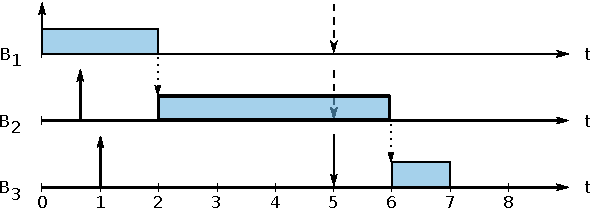
\includegraphics[scale=1.00]{images/producer-worker-consumer}
  \caption{Et generator/arbejder/forbruger -netværk. Kasserne repræsentere det tidsrum hvor processerne bliver bearbejdet. En pil op indikere hvornår processen er klar til at blive eksekveret. En pil ned indikere en deadline for processen. De stiplede pile i proces B$_1$ og B$_2$ til tiden t$=5$ viser en kunstig prioritet på baggrund af B$_3$'s deadline. Den lille stiplede pil mellem  B$_1$ og B$_2$ i t$=2$ og mellem B$_2$ og B$_3$ i t$=6$ viser kommunikation mellem processerne.}
  \label{fig:producer-worker-consumer}
  \end{center}
\end{figure}
\fxnote{Skriv på figurene hvem der er generator/arbejder/forbruger}
\begin{figure}
 \begin{center}
  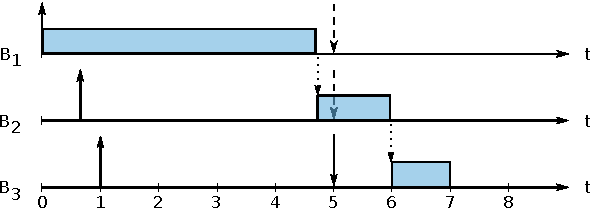
\includegraphics[scale=1.00]{images/producer-worker-consumer2}
  \caption{Samme netværk som i \autoref{fig:producer-worker-consumer}, men i dette tilfælde venter B$_2$  på data fra B$_1$ i hovedparten af tiden inden en deadline.}
  \label{fig:producer-worker-consumer2}
  \end{center}
\end{figure}


Der er dog ikke sikkert at en deadlineException i processer der har nedarvet en prioritet, er med til klarlægge hvilke processer der har brugt al tiden, og derfor bærer skylden for at en deadline ikke blev overholdt. \CRef{fig:producer-worker-consumer2} viser et eksempel på dette. Netværket er opsat som i \autoref{fig:producer-worker-consumer}, men i dette tilfælde bruger generatorprocessen (B$_1$) al tiden, og data bliver først sendt fra $B_1$ umiddelbart før en overskridelse af deadlinen. For en udvikler  vil det fremgå, som var det arbejderprocessen (B$_2$), der er ansvarlig for overskridelsen ligesom i \autoref{fig:producer-worker-consumer}, og ikke generatorprocessen $B_1$, som i dette eksempel brugte det meste af tiden. Dermed mister \code{deadlineException} sin troværdighed, og brugbarhed til at identificere hvor i netværket tiden bruges. 

Et andet problem ved at lade den aktive proces kaste en \code{deadlineException} er, at det vil pålægge udvikleren et væsentligt større arbejde med at håndtere disse exceptions. Såfremt vi implementerer det, kan enhver proces, der kan arve en prioritet via prioritetsnedarvning, kaste en exception. Det er ikke nødvendigvis klart gennemskueligt hvilke processer det vil være, hvorved udvikleren kan have svært ved at sikre ordentlig fejlhåndtering. Yderligere vil det medføre at excpetions kan kastes udenfor den kontekst de er relateret til, hvorved det kan være umuligt at håndtere dem korrekt.  

På baggrund af de opstillede fordele og ulemper, har vi valgt at kun processer med en eksplicit deadline, har mulighed for at kaste en \code{deadlineException}. Processer, der nedarver en prioritet, bliver planlagt i henhold til den højeste prioritet, de har, og vil altid  gøre arbejdet færdigt. En proces skal dermed kunne adskille sin egen deadline fra den prioritet, som den skal planlægges med, selv om de to værdier i en stor del af tiden vil være det samme.

En deadline er dermed en variabel der kun kan sættes af udvikleren og det er kun på baggrund af denne deadline at  processen skal kaste en \code{deadlineException}.

For at  \sched en kan udvælge processer introduceres prioritet, der som standard er det samme tal som deadlinen. For at kunne håndtere flere niveauer af prioritetsnedarvning,  gemmes prioriteten i en  liste kaldet \code{inherit\_priotity}. Denne liste af prioriteter  indeholder indledningsvis kun en prioritet som er deadlinen sat af udvikleren. Når andre processer  midlertidigt ønsker at ændre en proces' prioritet, tilføjes den til listen. Ved at bruge en liste i stedet for blot en variabel, har processen mulighed for at blive opprioriteret flere gange og derefter trinvist vende tilbage til de tidligere niveauer.

Når \sched en placerer processen i hhv. \code{has\_priority} og \code{no\_priority} hobene, bruges blot den mindste prioritet i listen af nedarvede prioriteter ihht. vores implementering af \sched en. Dette medfører, at når en proces efterfølgende  får ændret sin liste af prioriteter, skal processen genplanlægges for at sikre, at den placeres korrekt i min-hoben i \sched en. 

\subsection{Kanaler}
I \pycsp findes der kun kanaler af typen \code{Any-To-Any}, og derfor kan der altid  være et vilkårligt antal kanalender i hver ende af kanalen, der kan være klar til at kommunikere. Vi skal derfor foretage en ændring, så kommunikationen mellem kanalenderne altid foregår mellem de højst prioriterede processer. 

I greenletsversionen foregår udvælgelsen af kanalender til kommunikation ved hjælp af funktionen \code{match}, der udnytter at  hver kanal vedligeholder to lister af processer for hhv. de processer, der ønsker at sende, og modtage data på kanalen. Når en proces eks. ønsker at modtage data, tilføjer den sig selv til listen af processer, der ønsker at modtage, og prøver derefter i \code{match} funktionen at finde en proces, der vil sende data. Er der ingen processer, der venter på at sende data, venter processen på, at en proces melder sig klar til at sende data, ved at kalde \code{match}. Til hver vellykket kommunikation af data vil \code{match} altid blive kaldt to gange, hvor kun den sidste vil resultere i at kommunikationen lykkes.

Ideen bag funktionen \code{match} er enkel og  udnytter, at \code{greenlets}-versionen er enkelttrådet, så hver proces kan løbe listerne igennem, uden andre processer ændre på listernes tilstand.  Vi er kommet frem til, at  en simpel sortering af listerne ud fra processernes interne prioritet vil resultere i, at det altid er den højst prioriterede proces der indgår i kommunikationen. Den ændrede \code{match} kan ses i \cref{lst:match}, hvor det kun er linje 119 og 120 der er ændret.

\begin{lstlisting}[firstnumber=117 ,float=hbtp, label=lst:match, caption=Funktionen \code{match} der sorterer kanalrequests.]
def match(self):        
    if self.readqueue and self.writequeue:
        self.readqueue.sort(key=lambda channelReq:channelReq.process.internal_priority)
        self.writequeue.sort(key=lambda channelReq:channelReq.process.internal_priority)
        for w in self.writequeue:
            for r in self.readqueue:
                if w.offer(r):
                    return       
\end{lstlisting}

Funktionen \code{match} vil blive kaldt en gang for hver proces der ønsker at kommunikere, og derfor vil det kun være det sidste element i listen som ikke er sorteret korrekt ved hver kald af \code{match}. Desuden vil der altid i den ene liste maksimalt være på et element. Bemærk desuden at listerne er sorteret så værdien af den interne prioritet er stigende, og derfor er det processen med lavest værdi, der først bliver udvalgt til et match, i overensstemmelse med repræsentationen af prioriteter som nævnt i afsnittet ``Ændringer i \sched en'' %\vpageref{sec:sched-changes}.
på side \vpageref{sec:sched-changes}.
\fxerror{ret til vpageref}


\subsection{Prioritetsnedarvning}
\label{sec:deadline-implementation-priorityinheritance}
Prioritet i et RTP system skal ses i forhold til alle processers prioritet. En proces kan derfor ikke i sig selv have en absolut høj prioritet, men kun have høj prioritet ifht. de andre processers prioritet. Ved at give en høj prioritet til  en proces, vil dette dermed  indirekte sænke de andre processers prioritet, et fænomen vi vil kalde ``prioritetsdevaluering``.

For at minimere prioritetsdevaluering i forbindelse med prioritetsnedarvning, ønsker vi at minimere den tid en proces har en kunstigt høj prioritet, og at minimere antallet af processer, hvis prioritet øges. 

Som vi er kommet frem til i \cref{sec:rtp-pycsp-nedarvning}, skal  der foregå  prioritetsnedarvning i forbindelse med kommunikation, hvis der ikke findes nogle processer, der umiddelbart er klar til at kommunikere.  I \pycsp kan man umiddelbart evaluere, om der er processer klar til at kommunikere over en given kanal. Det skyldes, at processer der ønsker kommunikation befinder sig i listerne \code{readqueue} og \code{writequeue}. Hvis ingen processer ønsker at kommunikere, kan man dog ikke finde de processer som potentielt kan indgå i kommunikation.
Vi må derfor udvide kanalerne i RTP versionen med to lister, \code{readerprocesses} og \code{writerprocesses}, der består af de processer, der potentielt kan sende og modtage data over kanalen. Vi håndterer vedligeholdelsen af disse lister, ved at hver proces ved opstart tilføjer sig selv til de kanaler, den har mulighed for at kommunikere over. Et oplagt sted at implementere denne funktionalitet er i processens  \code{\_\_init\_\_}  funktion, da alle kanalender som denne proces potentielt kan kommunikere over, findes som argument til  \code{\_\_init\_\_} funktionen. \CRef{lst:process-init} viser udvidelsen af funktionen, hvor argumenterne gennemløbes, mens der ledes efter kanaler, som processen skal registreres i.

\begin{lstlisting}[firstnumber=29 ,float=hbtp, label=lst:process-init, caption=Uddrag af \code{Process}' \code{\_\_init\_\_}funktion]
for arg in args:
    if isinstance(arg, pycsp.greenlets.channelend.ChannelEndRead):
        arg.channel._addReaderProcess(self)
    if isinstance(arg, pycsp.greenlets.channelend.ChannelEndWrite):
        arg.channel._addWriterProcess(self)  
\end{lstlisting}

Kanaler kender nu  både de processer, der på et specifikt tidspunkt ønsker at kommunikere vha. listerne \code{readqueue} og \code{writequeue}, og de processer, der potentielt vil kunne kommunikere vha. listerne \code{readerprocesses} og \code{writerprocesses}. Processer der ønsker at kommunikere kan, som normalt umiddelbart evaluere om det er muligt; såfremt det ikke er muligt, kan den nu evaluere hvilke processers prioritet den kan øge, for at bringe dem i en tilstand hvor de kan indgå i den ønskede kommunikation. 

Funktionaliteten til prioritetsnedarvning skal implementeres i de to interne kommunikationfunktioner  \code{\_read} og \code{\_write}. Fordelen ved at placere prioritetsnedarvning i disse to funktioner er, at de bruges af processerne både i forbindelse med normal blokerende kommunikation og i forbindelse med kommunikation i \code{alternation}. Vi har udvidet funktionerne med følgende liste af begivenheder:
\begin{itemize}
\tightlist
	\item Undersøg om processen opfylder kriterierne for at starte en prioritetsnedarvning.
	\item Forhøj prioriteterne for de potentielle processer i enten \code{readerprocesses} eller \code{writer\-processes}.
	\item Umiddelbart efter kommunikationen nedprioriteres de processer, man midlertidigt har øget prioriteterne på.
\end{itemize}

Som beskrevet er det vigtigt, at vi igennem hele designet forsøger at begrænse mængden af prioritetsnedarvningen, og derfor har vi tilføjet en række egenskaber, der skal være indfriet, før prioritetsnedarvning forsøges. Disse er: processen skal have en prioritet, enten direkte eller efter en nedarvning; kanalen må ikke være klar til kommunikation, hvilket vil sige, at hvis processen ønsker at skrive, må der ikke findes en proces, der er klar til at modtage data; endeligt skal processen ikke have overskredet sin egen deadline, da denne til slut blot vil kaste en exception, og hele prioritetsnedarvningen vil være irrelevant.

Selve prioritetsforhøjelsen og den senere nedprioritering er simpel, da processen blot sender sin prioritet til alle processerne i den relevante liste dvs. \code{writerprocesses} for  \code{\_read} funktionen og vice versa. Hvis en proces modtager en lavere prioritet end dens egen prioritet, ses der bort fra hhv. op- og nedjusteringen, så en prioritetsnedarvning ikke resulterer i en forringelse af prioritet. 

\subsection{\code{Alternation}}

Som nævnt i afsnit \cref{misc:kanal-prioritet} har vi behov for at kunne tilknytte en prioritet til en kanal for at kunne håndtere udvælgelse i \code{alternations}. Vi har allerede prioriteter for processer og ønsker, at kanalernes prioritet skal defineres på baggrund af hvilke processer, der er tilknyttet kanalen. Vi skal kunne håndtere både input- og output-guards og ønsker seperate prioriteter for disse. Vi tilknytter derfor to prioriteter til hver kanal. De to prioriteter er sat som  de højst prioriterede processer, der er klar til at hhv. modtage og sende data. En kanals prioritet er derfor ikke fast som for processerne, hvor de får sat en prioritet (der dog kan ændres med prioritetsnedarvning), men nærmere en emuleret prioritet, som ændre sig baseret på alle processernes tilstand. 

Til at implementere de to prioriteter introduceres  to hjælpefunktioner, der løber hhv. \code{readqueue} og \code{writequeue} igennem og  finder den højst prioriterede proces, der er villig til hhv. at sende og modtage data. Når  \code{alternation} ønsker at finde prioriteten for en kanal, kigger den på om kanalen i \code{alternation} er tilknyttet en output- eller inputguard og finder den korrekte prioritet.



%\input{../test.tex}
\newpage
%\input{../konklusion.tex}

%\input{../jxta-services}

%%%%%%%%%%%%%%%%%%%%%%%%%%%%%%%%%%%%%%%%%%%%%%%%%%%%%%%%%%%%%%%%%%%%%%
%\input{../dibs} / skal det bruges og hvor?

\newpage
\backmatter
%\appendix
%\chapter{Billag}

%\pagenumbering{roman}
%\restorepagenumber

\linespread{1}
\printbibliography

%\chapter{Testresultater}
\thispagestyle{empty}

\section{Testresultater for \des}
\label{app:des-test}
\begin{longtable}{lr}
   	\toprule
    \mc{Test} & \mc{Resultat} \\
    \midrule
    \endfirsthead 
    \toprule
    \mc{Test} & \mc{Resultat} \\
    \midrule
    \endhead % slut efterfølgende headere
    \bottomrule
    \multicolumn{2}{r}{\textit{fortsættes}}
    \endfoot % slut footer
    \bottomrule
    \endlastfoot % slut sidste footer
    Doctest: simulation.Simulation & ok\\
    Doctest: simulation.io & ok\\
    Doctest: guard.testsuite & ok\\
    Doctest: alternation.Alternation & ok\\
    Doctest: alternation.testsuite & ok\\
    Doctest: channel.Channel & ok\\
    Doctest: channel.testsuite & ok\\
    Doctest: process.Parallel & ok\\
    Doctest: process.Spawn & ok\\
    Doctest: process.test\_suite & ok\\
    test\_alternation (test\_simulation.SimulationTestCase) & ok\\
    test\_buffer (test\_simulation.SimulationTestCase) & ok\\
    test\_buffered\_channels (test\_simulation.SimulationTestCase) & ok\\
    test\_decompose (test\_simulation.SimulationTestCase) & ok\\
    test\_io (test\_simulation.SimulationTestCase) & ok\\
    test\_timers1 (test\_simulation.SimulationTestCase) & ok\\
    test\_timers2 (test\_simulation.SimulationTestCase) & ok\\
    test\_timers3 (test\_simulation.SimulationTestCase) & ok\\
    test\_timers\_time\_in\_past (test\_simulation.SimulationTestCase) & ok\\
    test\_wait (test\_io.TestCase) & ok\\
\end{longtable}


\newpage
\section{Testresultater for RTP}
\label{app:rtp-test}
\fxnote{RS: ret stavefejl og sørg for at de to tabeller er formatteret ens}
\begin{longtable}{lr}
   	\toprule
    \mc{Test} & \mc{Resultat} \\
    \midrule
    \endfirsthead 
    \toprule
    \mc{Test} & \mc{Resultat} \\
    \midrule
    \endhead % slut efterfølgende headere
    \bottomrule
    \multicolumn{2}{r}{\textit{fortsættes}}
    \endfoot % slut footer
    \bottomrule
    \endlastfoot % slut sidste footer
test\_Alternation  & ok\\
test\_AlternationChoiseReader  & ok \\
test\_AlternationChoiseWriter  & ok \\
test\_AlternationExecuteReadDeadline  & ok\\
test\_AlternationExecuteSkipDeadline  & ok\\
test\_AlternationExecuteTimeoutDeadline  & ok \\
test\_AlternationExecuteWriteDeadline  & ok \\
test\_Alternationchoise1Deadline  & ok \\
test\_Alternationchoise2Deadline  & ok \\
test\_ChoisemultipleReader  & ok \\
test\_ChoisemultipleReader2  & ok \\
test\_ChoisemultipleWriter  & ok\\
test\_PoisonAndDeadline1  & ok\\
test\_PoisonAndDeadline2  & ok\\
test\_Reader\_Inheritance  & ok\\
test\_RetireAndDeadline  & ok\\
test\_Writer\_Inheritance  & ok\\
test\_channelpriority\_from\_low\_deadline  & ok\\
test\_channelpriority\_from\_low\_deadline2  & ok\\
test\_channelpriority\_from\_no\_deadline  & ok\\
test\_channelpriority\_from\_no\_deadline2  & ok\\
test\_readDeadline  &ok\\
test\_writeDeadline  & ok\\
test\_xreset\_inheritance  & ok\\
test\_xreset\_inheritance\_from\_two\_step  & FAIL\\
\end{longtable}



\chapter{Eksempler}
\section{Eksempler til \des}
\lstinputlisting[label=code_wator, caption=WaTor i simulerings-versionen]{../projects/wator/wator-des.py}
\lstinputlisting[label=code_simpel_bank, caption=Simpelt bankeksempel i simulerings-versionen]{../projects/bank/src/bank03.py}
\lstinputlisting[label=code_avanceret_bank, caption=Avanceret bankeksempel i simulerings-versionen]{../projects/bank/src/bank04.py}

\section{Eksempler til RTP}  
\lstinputlisting[label=code_slagteri, caption=Slagterieksemplet RTP-versionen]{../projects/porks-rtp/porks-rtp.py}
\section{Eksempler til IP}  
\lstinputlisting[label=code_ur, caption=Ureksemplet RTP-versionen]{../projects/watch-ip/watch.py}

 %Fjern %, så vedhæftes bilag (i final)
\end{document}
